\section{Resultados}
\label{sec:resultados}

Todas as métricas de ponta a ponta e orientação foram reverificadas com o script
reprodutível \texttt{scripts/eval\_metrics.py} (seed fixa, $N=60$ imagens amostradas
aleatoriamente do dataset). Métricas do classificador de tipo de peça e cor foram
avaliadas isolando o classificador da pipeline clássica, ou seja, fornecendo a ocupação
do gabarito (GT) como entrada --- isso evita que erros de ocupação/cantos se propaguem
para a avaliação do classificador de tipo.

\subsection{Detecção de ocupação (pipeline clássica, ponta a ponta)}

\begin{table}[H]
\centering
\caption{Ocupação --- 60 imagens, cantos detectados automaticamente (Hough).}
\begin{tabular}{@{}lrrrr@{}}
\toprule
Métrica & Média & Mediana & Mín. & Máx. \\
\midrule
Acurácia & 64,5\% & 59,4\% & 34,4\% & 98,4\% \\
Precisão & 59,8\% & 58,8\% & 0\% & 100\% \\
Recall   & \textbf{70,2\%} & 79,6\% & 0\% & 100\% \\
F1       & 62,7\% & 66,7\% & 0\% & 98,4\% \\
\bottomrule
\end{tabular}
\end{table}

Com \textbf{cantos do gabarito} (isolando o erro de detecção de cantos do restante da
pipeline), o F1 de ocupação sobe para \textbf{86,3\%} --- confirmando que o gargalo
principal do sistema é a detecção automática dos 4 cantos do tabuleiro, e não a votação
de características de ocupação em si. O recall consistentemente maior que a precisão
indica que o pipeline tende a \textbf{superestimar} a ocupação (marcar casas vazias como
ocupadas) devido ao baixo contraste madeira-sobre-madeira, mais do que a perder peças
existentes.

\subsection{Classificação de cor}

Avaliada com cantos do gabarito sobre 200 imagens, a classificação de cor por limiar
fixo do canal V (HSV) atinge \textbf{82,5\%} de acerto geral. Cerca de 38\% das imagens
são ``fáceis'' (acerto $\geq$ 90\%, bom contraste peça-fundo); 18\% são ``difíceis''
(acerto $<$ 70\%), tipicamente por sombra projetada ou peça escura sobre casa escura, onde
o limiar fixo de brilho falha.

\subsection{Classificação de tipo de peça (ResNet-34)}

Avaliada em 50 imagens com ocupação do gabarito (isola o classificador do restante da
pipeline; FN = FP = 0 por construção, já que a ocupação é fornecida):

\begin{table}[H]
\centering
\caption{Classificador de tipo de peça --- métricas globais.}
\begin{tabular}{@{}lr@{}}
\toprule
Métrica & Valor \\
\midrule
Precisão & 91,0\% \\
Recall   & 91,0\% \\
F1-score & \textbf{91,0\%} \\
Peças corretas (tipo + posição) & 1\,412 \\
Tipo errado (posição certa)     & 140 \\
\bottomrule
\end{tabular}
\end{table}

\begin{table}[H]
\centering
\caption{Acurácia por classe de peça.}
\begin{tabular}{@{}lrl@{}}
\toprule
Classe & Acurácia & Observação \\
\midrule
knight\_b & \textbf{96,4\%} & silhueta do cavalo é distintiva \\
pawn\_b   & 96,3\% & classe mais representada \\
knight\_w & 95,9\% & --- \\
pawn\_w   & 93,8\% & --- \\
queen\_w  & 90,8\% & melhorou de 27,7\% para 90,8\% com \textit{fine-tuning} \\
rook\_w   & 90,1\% & --- \\
rook\_b   & 89,2\% & --- \\
king\_w   & 89,7\% & --- \\
bishop\_w & 87,6\% & --- \\
bishop\_b & 88,2\% & --- \\
queen\_b  & 87,8\% & --- \\
king\_b   & \textbf{84,5\%} & classe mais difícil; efeito residual do desbalanceamento \\
\bottomrule
\end{tabular}
\end{table}

Quando avaliado conjuntamente com a classificação de cor (tipo + cor, ocupação do
gabarito, $N=60$), o acerto é de \textbf{93,0\%}, consistente com o F1 de 91\% medido
isoladamente para o tipo.

\begin{figure}[H]
  \centering
  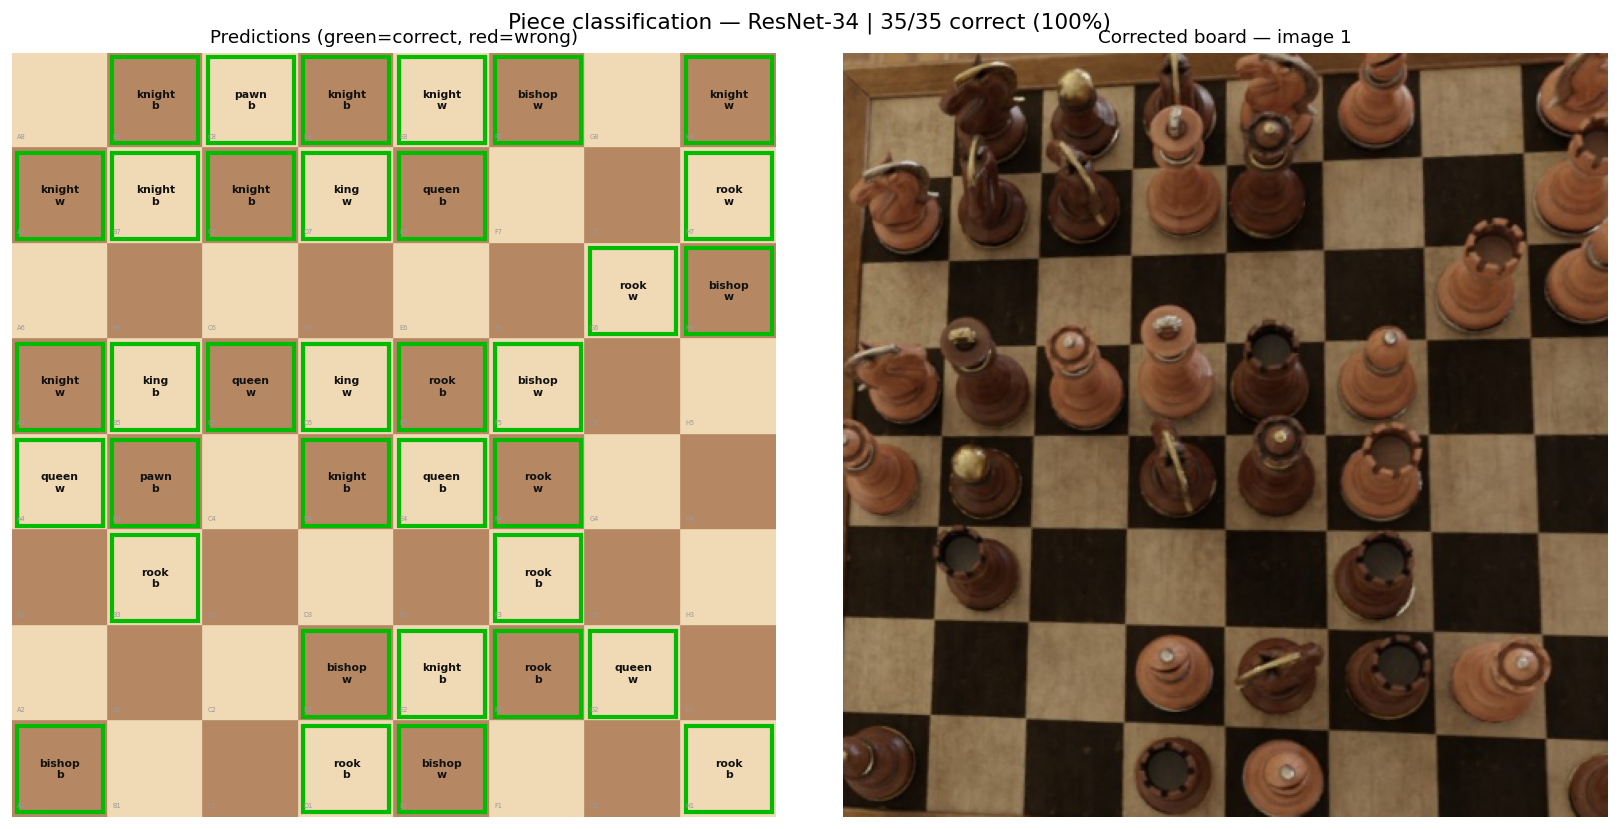
\includegraphics[width=0.55\textwidth]{../../andamento/images/15_piece_classification_result.png}
  \caption{Exemplo de leitura completa de um tabuleiro: 35/35 peças classificadas
    corretamente.}
\end{figure}

\subsection{Orientação sem gabarito e leitura de ponta a ponta}

Sobre as mesmas 60 imagens, a estimativa de orientação sem gabarito
(\texttt{detect\_board\_rotation}) apresenta \textbf{0\% de erro de eixo} --- o
tabuleiro nunca é lido girado em $90\degree$ ou $270\degree$ --- mas, como discutido na
Seção~\ref{sec:fen-jogadas}, cerca de \textbf{42\%} das leituras totalmente automáticas
ficam invertidas em $180\degree$ devido à simetria de cor do tabuleiro sob essa rotação.
Isso não é contabilizado como erro de leitura, e sim reportado explicitamente como
ambiguidade inerente, resolvida com a apresentação de duas FENs candidatas.

\subsection{Síntese}

\begin{table}[H]
\centering
\caption{Resumo por componente da pipeline.}
\small
\begin{tabular}{@{}>{\raggedright\arraybackslash}p{3.2cm}>{\raggedright\arraybackslash}p{6cm}>{\raggedright\arraybackslash}p{4.8cm}@{}}
\toprule
Componente & Abordagem & Resultado \\
\midrule
Detecção do tabuleiro & Hough + homografia & Robusto; gargalo do sistema \\
Segmentação $8\times8$ & Divisão uniforme & Exato \\
Ocupação & Votação de características (clássico) & F1 = 62,7\% (86,3\% c/ cantos GT) \\
Cor da peça & Limiar fixo de brilho HSV (clássico) & 82,5\% \\
\textbf{Tipo da peça} & \textbf{ResNet-34 --- \textit{transfer learning} + \textit{fine-tuning}} & \textbf{F1 = 91,0\%} \\
FEN + jogadas & Regras determinísticas sobre \texttt{piece\_map} & Validado em casos controlados \\
\bottomrule
\end{tabular}
\end{table}

O classificador de tipo de peça, baseado em \textit{deep learning}, é hoje a etapa mais
precisa da pipeline --- superando a precisão da detecção clássica de ocupação. O gargalo
de ponta a ponta permanece na etapa puramente geométrica de detectar os 4 cantos do
tabuleiro sob baixo contraste.
